\section{Not Liouville's Theorem}
Science doesn't tell us much about whether or not Liouville liked cats but we do know that some people have used pictures of cat faces to illustrate the concept of phasespace area conservation. 
Here are a collection of cat drawings from the 742 class of 2020.

\begin{centering}
\begin{figure}\centering
	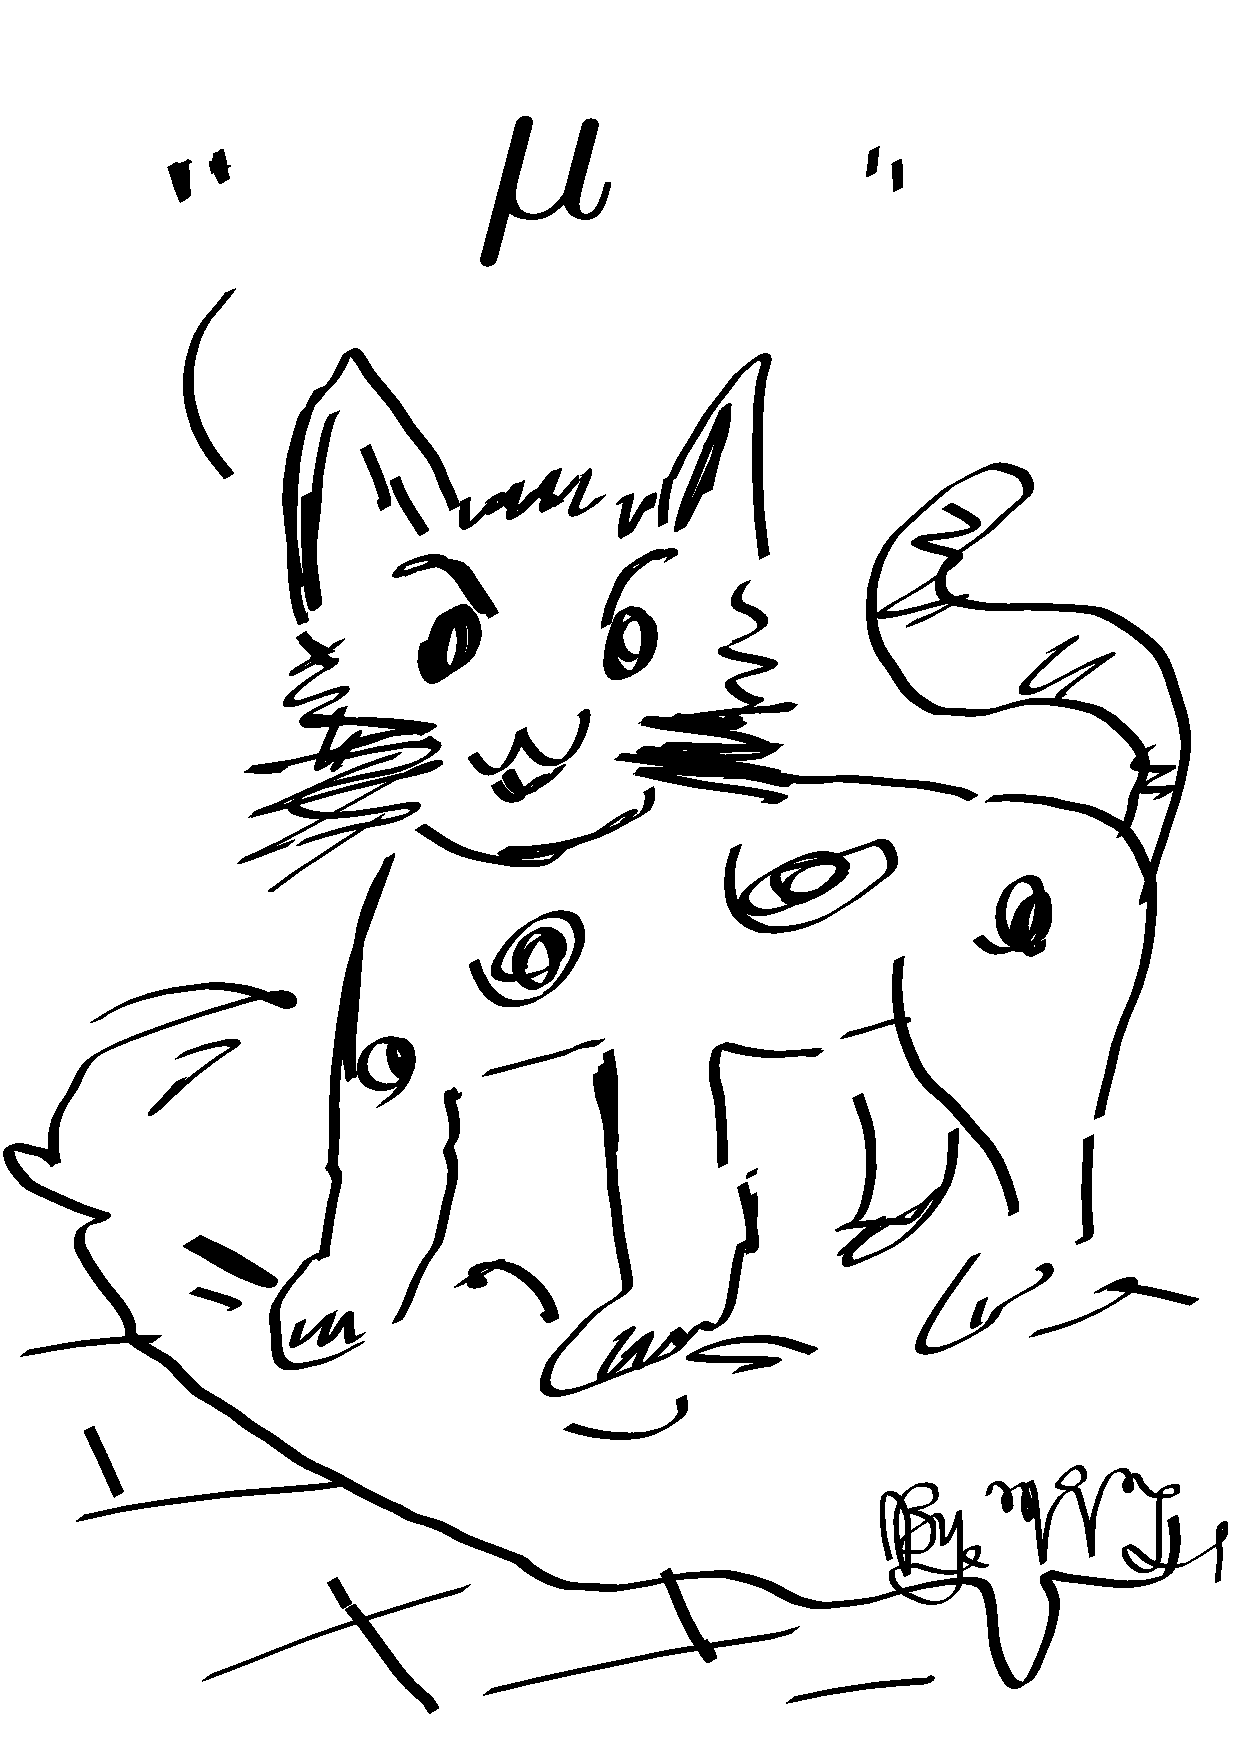
\includegraphics[width=8cm]{mucat.pdf}
  \caption{\textsl{"The $\mu$ cat"}, by Wang}
  \label{fig:cat1}
\end{figure}

\begin{figure}
	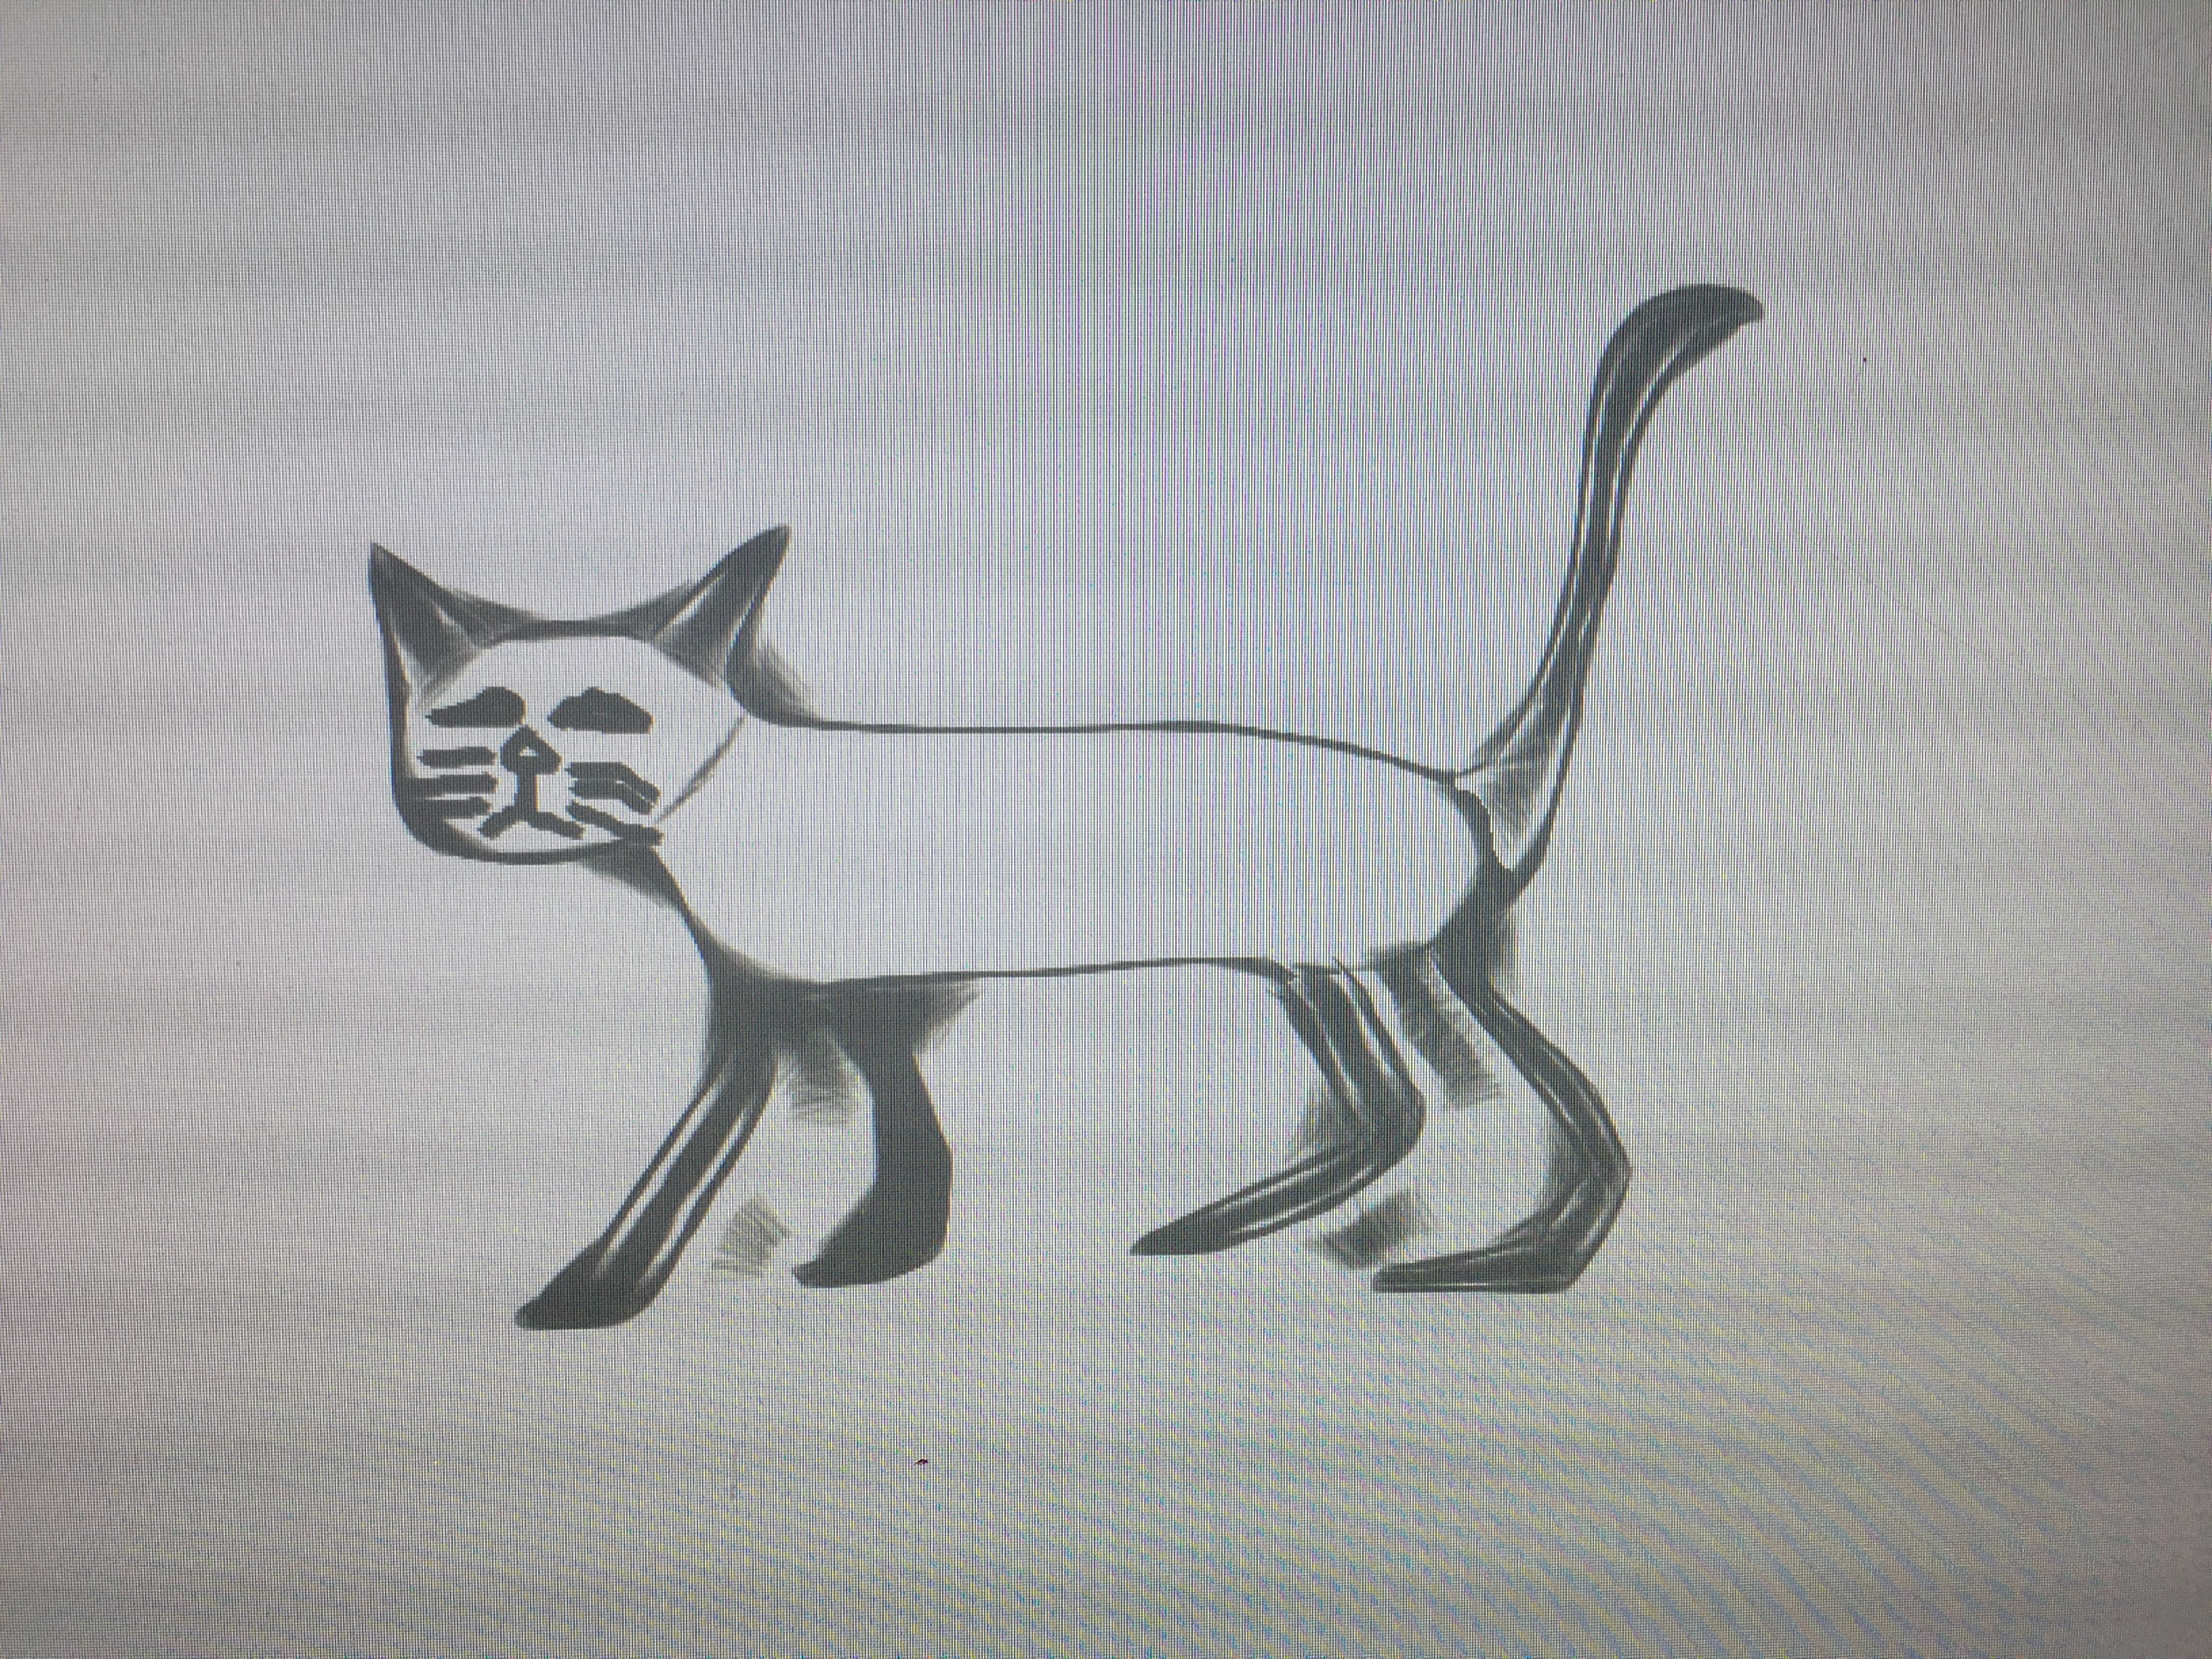
\includegraphics[width=8cm]{catsketch.pdf}
  \caption{Frazer's Cat Sketch}
  \label{fig:catsketch}
\end{figure}

\begin{figure}
	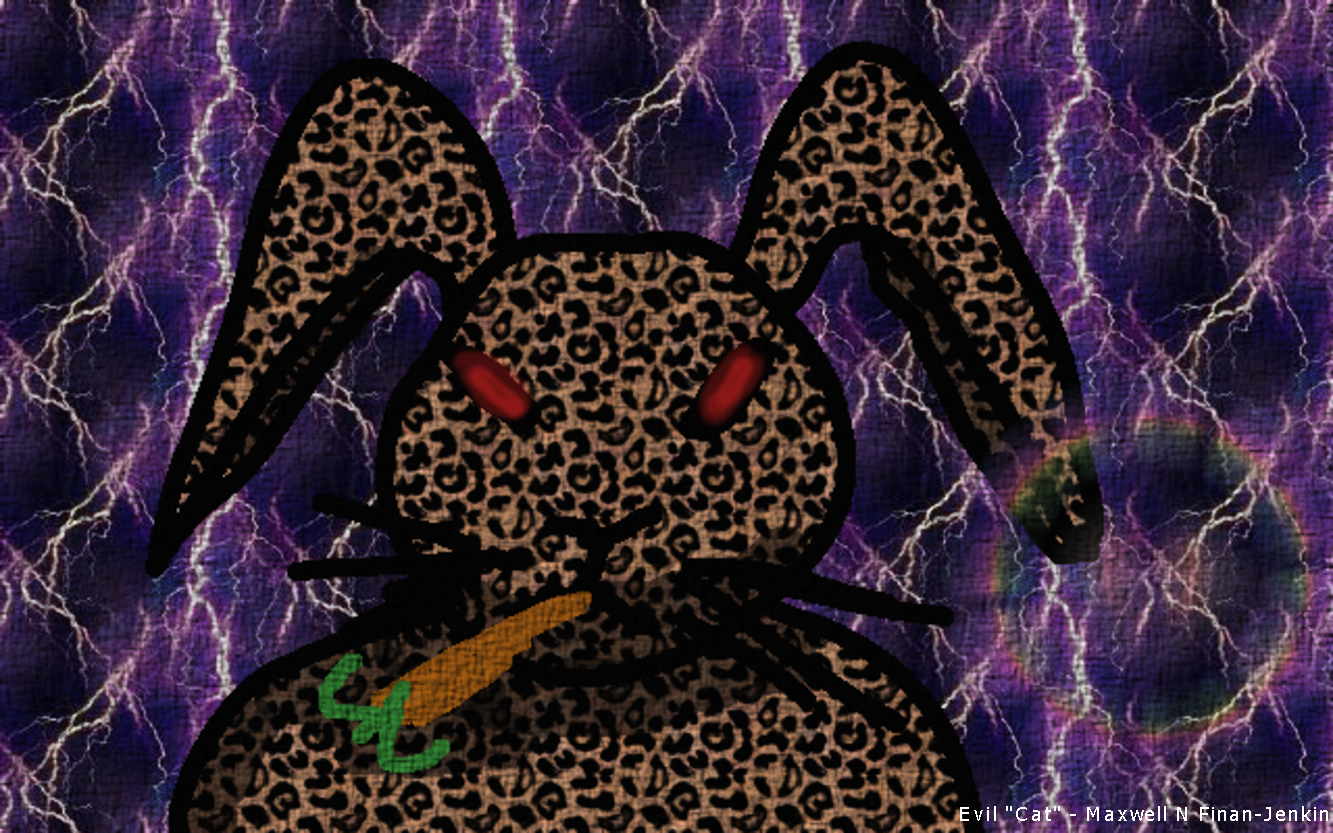
\includegraphics[width=8cm]{catto.pdf}
  \caption{An evil 'Cat' that Maxwell drew}
  \label{fig:catto}
\end{figure}



\begin{figure}
	\includegraphics[width=8cm]{cat1.pdf}
  \caption{A cat that Alex drew.}
  \label{fig:cat1}
\end{figure}



\begin{figure}
	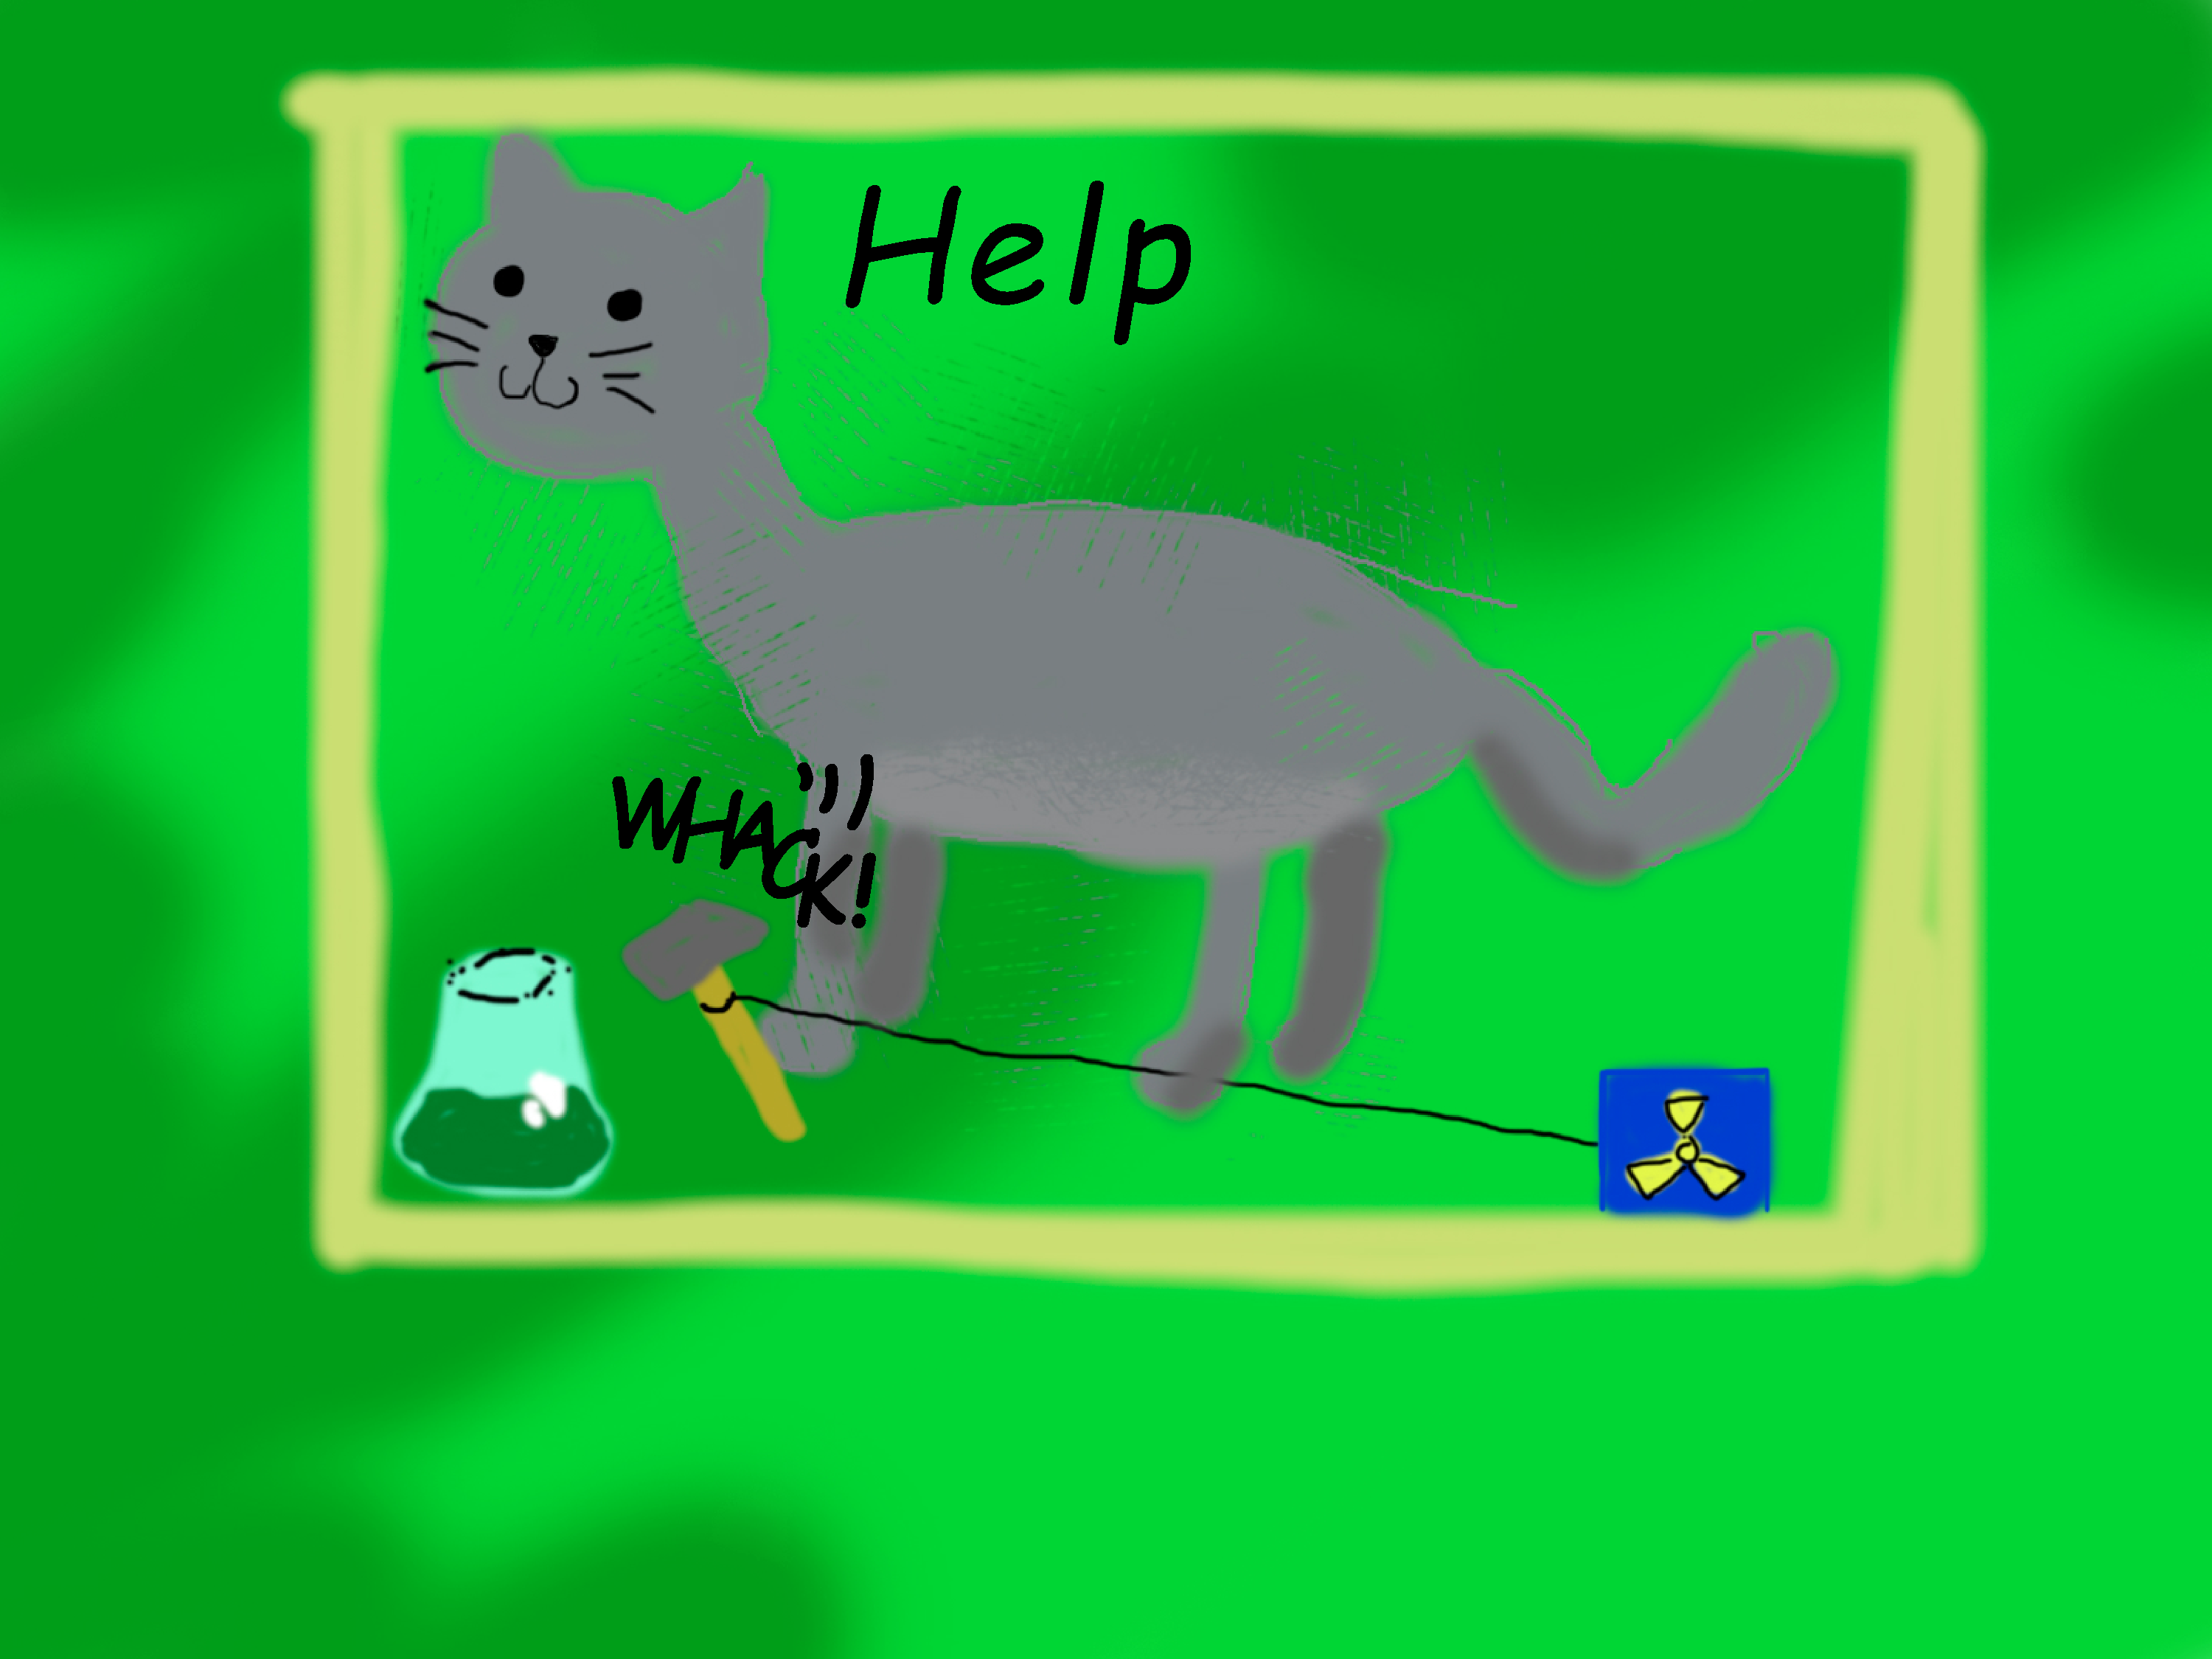
\includegraphics[width=8cm]{cat-gleb.pdf}
  \caption{let's be honest: it's probably dead. Gleb }
  \label{fig:cat1}
\end{figure}



\begin{figure}
	\includegraphics[width=8cm]{cat742afer228.pdf}
  \caption{A cat that Kamrun drew.}
  \label{Cat draw by Kamrun}
\end{figure}




\begin{figure} \centering
    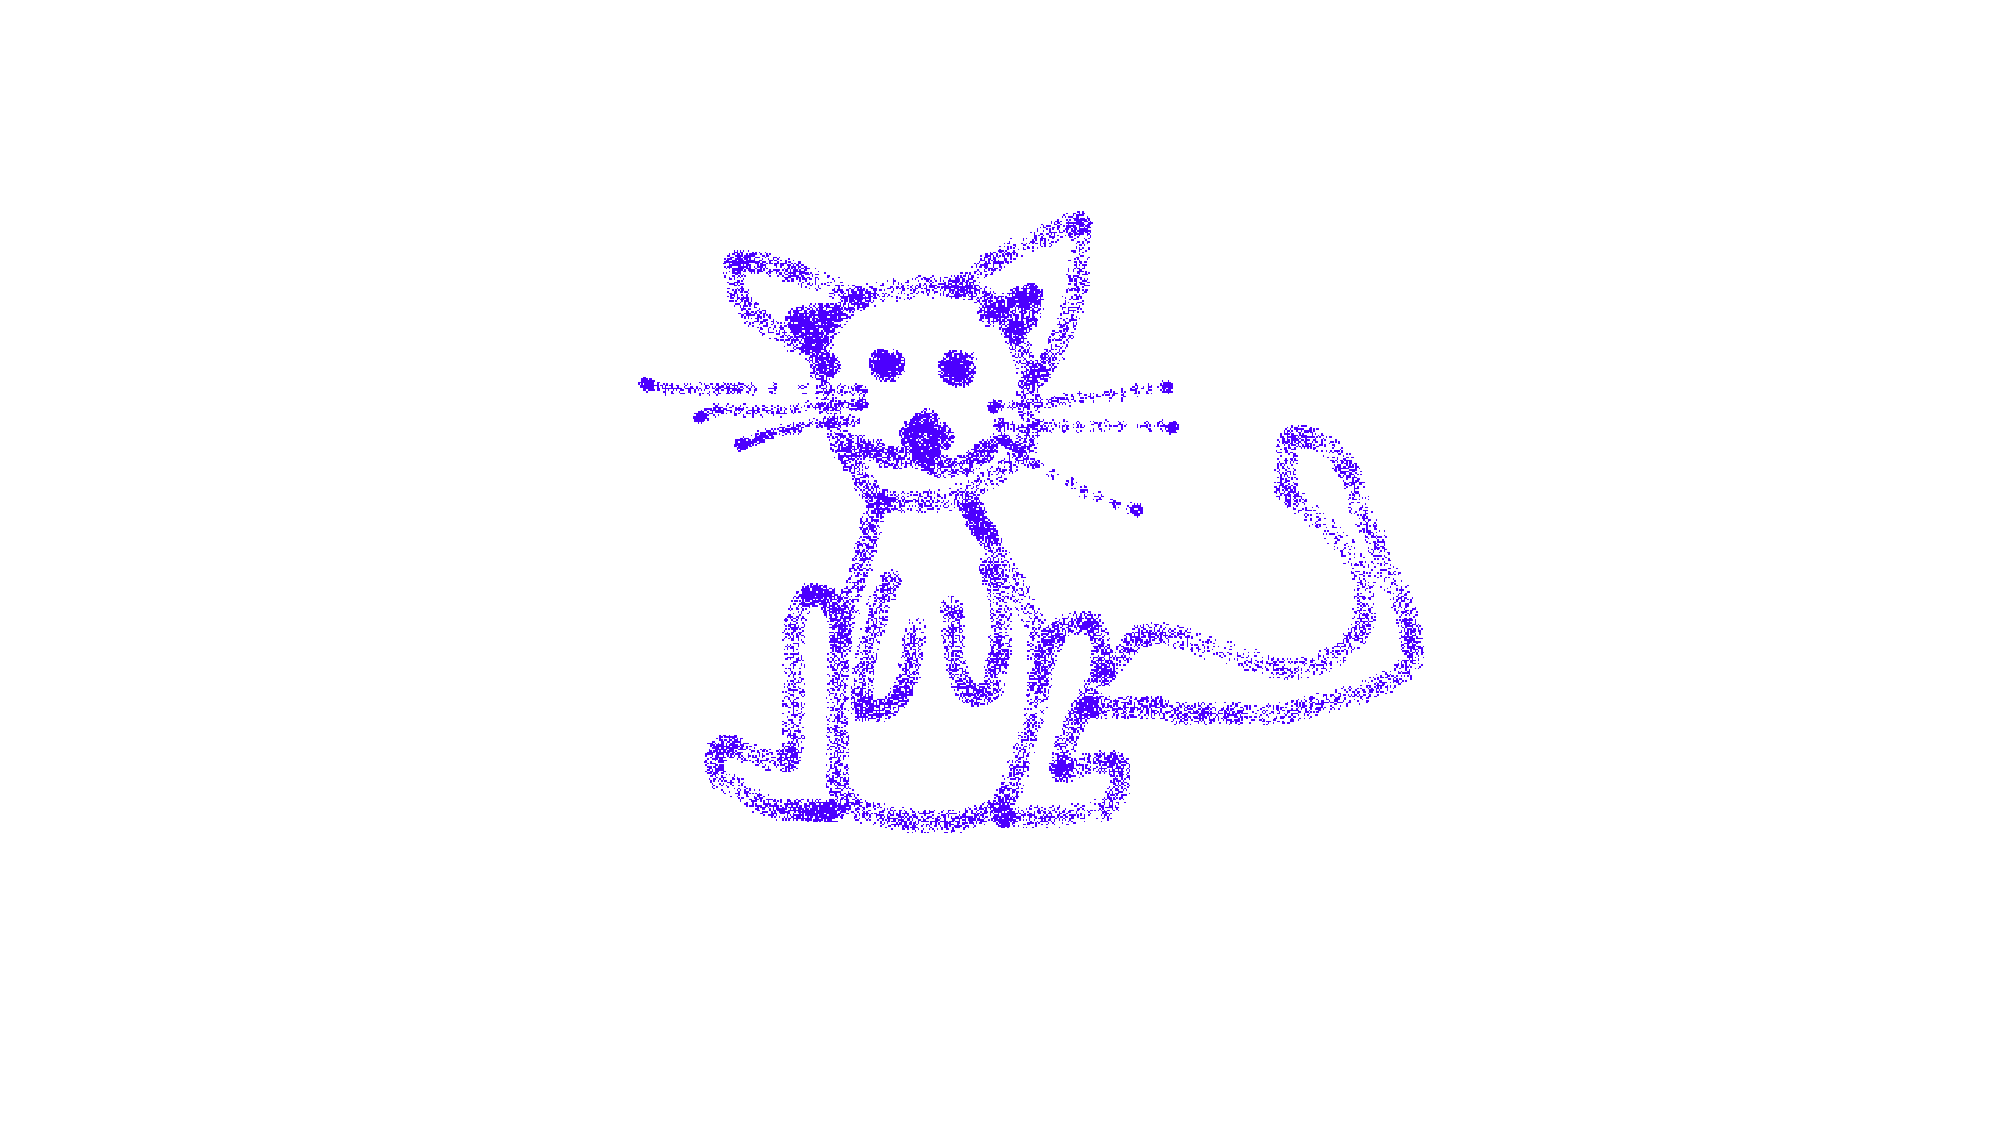
\includegraphics[width=8cm]{kat.pdf}
    \caption{\emph{``Kat"}, by Jasmine}
    \label{kat}
\end{figure}


\begin{figure}\centering
  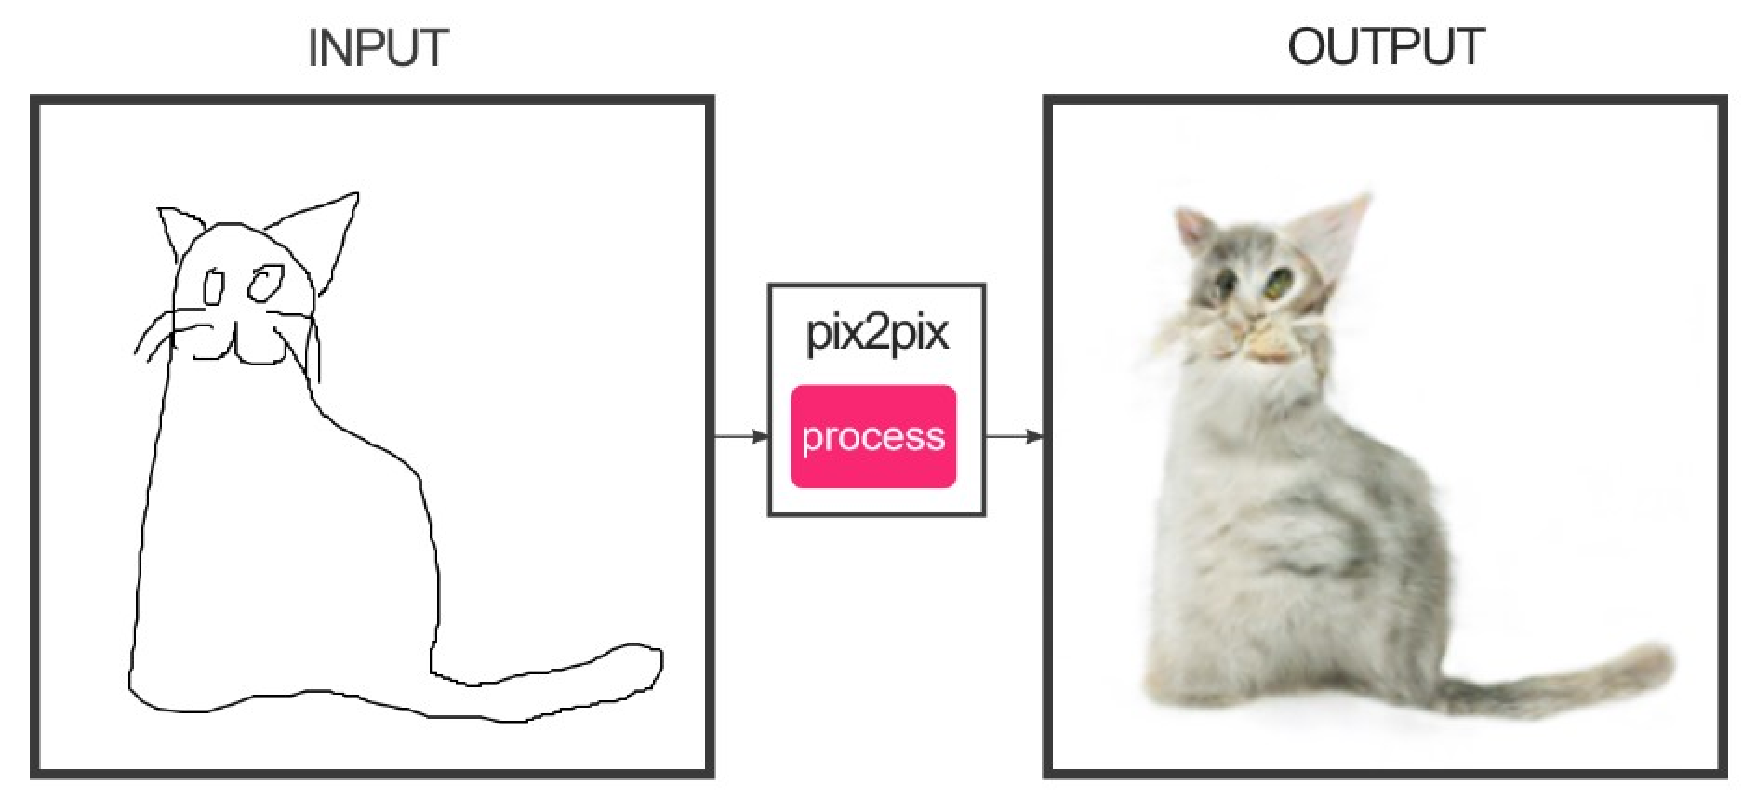
\includegraphics[width=8cm]{cat-fadiwassaf.pdf}
  \caption{I needed some help. Courtesy of edges2cats on https://affinelayer.com/pixsrv. - Fadi}
  \label{cat-fadi}
\end{figure}
\end{centering}


\clearpage
